\documentclass[tikz,border=5pt]{standalone}
\usepackage{tikz}
\usetikzlibrary{arrows.meta,calc}

\begin{document}
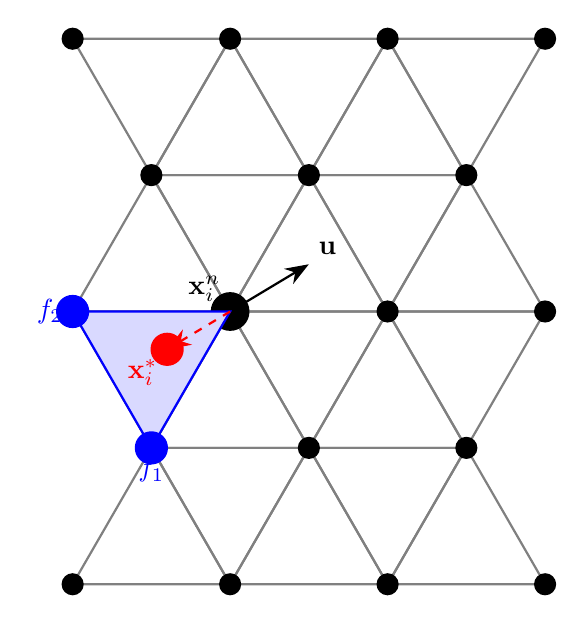
\begin{tikzpicture}[scale=2.0]

    % Define vertices of a fully triangular mesh (regular pattern)
    % Row 0
    \coordinate (A0) at (0,0);
    \coordinate (B0) at (1,0);
    \coordinate (C0) at (2,0);
    \coordinate (D0) at (3,0);
    % Row 1
    \coordinate (A1) at (0.5,0.866);
    \coordinate (B1) at (1.5,0.866);
    \coordinate (C1) at (2.5,0.866);
    % Row 2
    \coordinate (A2) at (0,1.732);
    \coordinate (B2) at (1,1.732);
    \coordinate (C2) at (2,1.732);
    \coordinate (D2) at (3,1.732);
    % Row 3
    \coordinate (A3) at (0.5,2.598);
    \coordinate (B3) at (1.5,2.598);
    \coordinate (C3) at (2.5,2.598);
    % Row 4
    \coordinate (A4) at (0,3.464);
    \coordinate (B4) at (1,3.464);
    \coordinate (C4) at (2,3.464);
    \coordinate (D4) at (3,3.464);

    % Draw triangular mesh - Row 0 to 1
    \draw[gray, thick] (A0) -- (B0) -- (A1) -- cycle;
    \draw[gray, thick] (B0) -- (C0) -- (B1) -- cycle;
    \draw[gray, thick] (C0) -- (D0) -- (C1) -- cycle;
    \draw[gray, thick] (B0) -- (B1) -- (A1) -- cycle;
    \draw[gray, thick] (C0) -- (C1) -- (B1) -- cycle;

    % Row 1 to 2
    \draw[gray, thick] (A1) -- (A2) -- (B2) -- cycle;
    \draw[gray, thick] (A1) -- (B2) -- (B1) -- cycle;
    \draw[gray, thick] (B1) -- (B2) -- (C2) -- cycle;
    \draw[gray, thick] (B1) -- (C2) -- (C1) -- cycle;
    \draw[gray, thick] (C1) -- (C2) -- (D2) -- cycle;

    % Row 2 to 3
    \draw[gray, thick] (A2) -- (B2) -- (A3) -- cycle;
    \draw[gray, thick] (B2) -- (C2) -- (B3) -- cycle;
    \draw[gray, thick] (C2) -- (D2) -- (C3) -- cycle;
    \draw[gray, thick] (B2) -- (B3) -- (A3) -- cycle;
    \draw[gray, thick] (C2) -- (C3) -- (B3) -- cycle;

    % Row 3 to 4
    \draw[gray, thick] (A3) -- (A4) -- (B4) -- cycle;
    \draw[gray, thick] (A3) -- (B4) -- (B3) -- cycle;
    \draw[gray, thick] (B3) -- (B4) -- (C4) -- cycle;
    \draw[gray, thick] (B3) -- (C4) -- (C3) -- cycle;
    \draw[gray, thick] (C3) -- (C4) -- (D4) -- cycle;

    % Draw all mesh vertices (black dots)
    \foreach \p in {A0,B0,C0,D0,A1,B1,C1,A2,B2,C2,D2,A3,B3,C3,A4,B4,C4,D4} {
        \fill[black] (\p) circle (2pt);
    }

    % Current point x_i^n (at vertex B2)
    \fill[black] (B2) circle (3.5pt);
    \node[above left] at (B2) {$\mathbf{x}_i^n$};

    % Velocity direction (pointing up-right)
    \coordinate (velDir) at (0.5, 0.3);
    \draw[-{Stealth[length=3mm]}, thick, black] (B2) -- ($(B2)+(velDir)$);
    \node[above right] at ($(B2)+(velDir)$) {$\mathbf{u}$};

    % Backtracking position x_i^* (opposite direction of velocity)
    \coordinate (BT) at ($(B2) - 0.8*(velDir)$);

    % Highlight interpolation triangle - the one containing BT (A1-A2-B2, left of B2)
    \fill[blue!15] (A1) -- (A2) -- (B2) -- cycle;
    \draw[blue, thick] (A1) -- (A2) -- (B2) -- cycle;

    % Draw backtracking point and line
    \fill[red] (BT) circle (3pt);
    \node[below left, red] at (BT) {$\mathbf{x}_i^*$};

    % Backtracking trajectory (STRAIGHT LINE - opposite to velocity)
    \draw[red, thick, dashed, -{Stealth[length=3mm]}] (B2) -- (BT);

    % Label interpolation points
    \fill[blue] (A1) circle (3pt);
    \fill[blue] (A2) circle (3pt);
    \node[blue, below] at (A1) {$f_1$};
    \node[blue, left] at (A2) {$f_2$};

\end{tikzpicture}
\end{document}
